\chapter{Foundations}\label{Chapter:Foundations}
\section{The Data Distribution Service}\label{Section:Intro}
Whether you are an experienced programmer or a newbie, it is highly likely 
that you have already experienced some form of \ac{Pub/Sub} -- 
%%
%%\todo[inline, caption={Actualize Intro}]{The description of DDS should be updated 
%% to put more emphasis on data sharing. I addition we should have some quick reference 
%% to MQTT, JMS,~\ldots}
%%
an abstraction for one-to-many communication that provides anonymous, 
decoupled,  and asynchronous communication between the publisher and 
its subscribers. \ac{Pub/Sub} is the abstraction behind many of the technologies 
used today to build and integrate distributed applications, such as, social 
application,  financial trading, etc., while maintaining their 
composing parts loosely coupled and independently evolvable.

Various implementations of the \ac{Pub/Sub} abstraction have emerged through time to 
address the needs of different application domains. \ac{DDS} is an \ac{OMG} 
standard for \ac{Pub/Sub} introduced in 2004 to address the data sharing needs 
of large scale mission- and business-critical applications. Today \ac{DDS} is 
one of the hot technologies at the heart of some of the most interesting \ac{IoT} and 
\ac{I2} applications.
 
At this point, to the question "What is DDS?" I can safely answer that it is 
a \ac{Pub/Sub} technology for ubiquitous, polyglot, efficient and secure data sharing. 
Another way of answering this question is that \ac{DDS} is \ac{Pub/Sub} on \textit{steroids}.


\section {The OMG DDS Standard}
The \ac{DDS} standards family is today composed, as shown in
Figure~\ref{Figure:DDS:Standard}, by the 
\ac{DDS} v1.2 API \cite{OMG:DDS:04} and the \ac{DDSI} (\ac{DDSI} v2.1) \cite{OMG:DDSI:06}. 
% \todo[inline, caption={Standard References}]{Standard References are out of date.}
The \ac{DDS} API standard guarantees source code portability across different vendor 
implementations, while the \ac{DDSI} standard ensures on the wire interoperability 
between DDS implementations from different vendors. The \ac{DDS} API standard defines several  different profiles (see Figure~\ref{Figure:DDS:Standard}) that enhance 
real-time pub/sub with content filtering and queries, temporal decoupling and automatic fail-over. 
%%
\begin{figure}[ht]
	\centering
	\includegraphics[scale=0.4]{figs/dds-standard.eps}
	\caption{The \ac{DDS} Standard.}
	\label{Figure:DDS:Standard}
\end{figure}
%%

The \ac{DDS} standard was formally adopted by the \ac{OMG} in 2004 and today it has 
become the established \ac{Pub/Sub} technology for distributing high volumes of data, 
dependably and with predictable low latency in applications such as, Smart Grids,
Smart Cities, Financial Trading, Air Traffic Control and Management,  High Performance Telemetry and  Large Scale Supervisory Systems. 

Now that I have given you an overall idea of what \ac{DDS} is and where it is being used 
let's try to see how it works.



\section {\ac{DDS} in  a Nutshell}
To explain \ac{DDS} I will take advantage of a running example that is 
simple and generic enough that you should easily relate to it. 
I will describe the example now and then use it to explain 
the various \ac{DDS} features throughout this tutorial. 
The example that I will use is the temperature monitoring and 
control system for a very large building. Each floor of 
the building has several rooms, each of which is equipped with 
a set of temperature and humidity sensors and one or more conditioners. 
The application is supposed to perform both monitoring for all the 
elements in the building as well as temperature and humidity control 
for each room. 

This application is a typical distributed monitoring and control 
application in which you have data telemetry from several sensors 
distributed over some spatial location and you also have the control 
action that has to be applied to the actuators--our conditioners. 

Now that we've created a task for you to solve, let's see what \ac{DDS} 
has to offer.

\subsection{Global Data Space}\index{Global Data Space}
The key abstraction at the foundation of \ac{GDS} is a fully 
distributed {\ac{GDS}. It is important to remark that the \ac{DDS} 
specification requires the implementation of the Global Data Space 
to be fully distributed to avoid point of failures and single point 
of bottleneck. Publishers and Subscribers can join or leave the \ac{GDS} 
at any point in time as they are dynamically discovered. The dynamic 
discovery of Publisher and Subscribers is performed by the \ac{GDS} 
and does not rely on any kind of centralized registry such as those 
found in other pub/sub technologies such as \ac{JMS}. Finally, 
I should mention that the \ac{GDS} also discovers application defined 
data types and propagates them as part of the discovery process.
%%
\begin{figure}[ht]
	\centering
	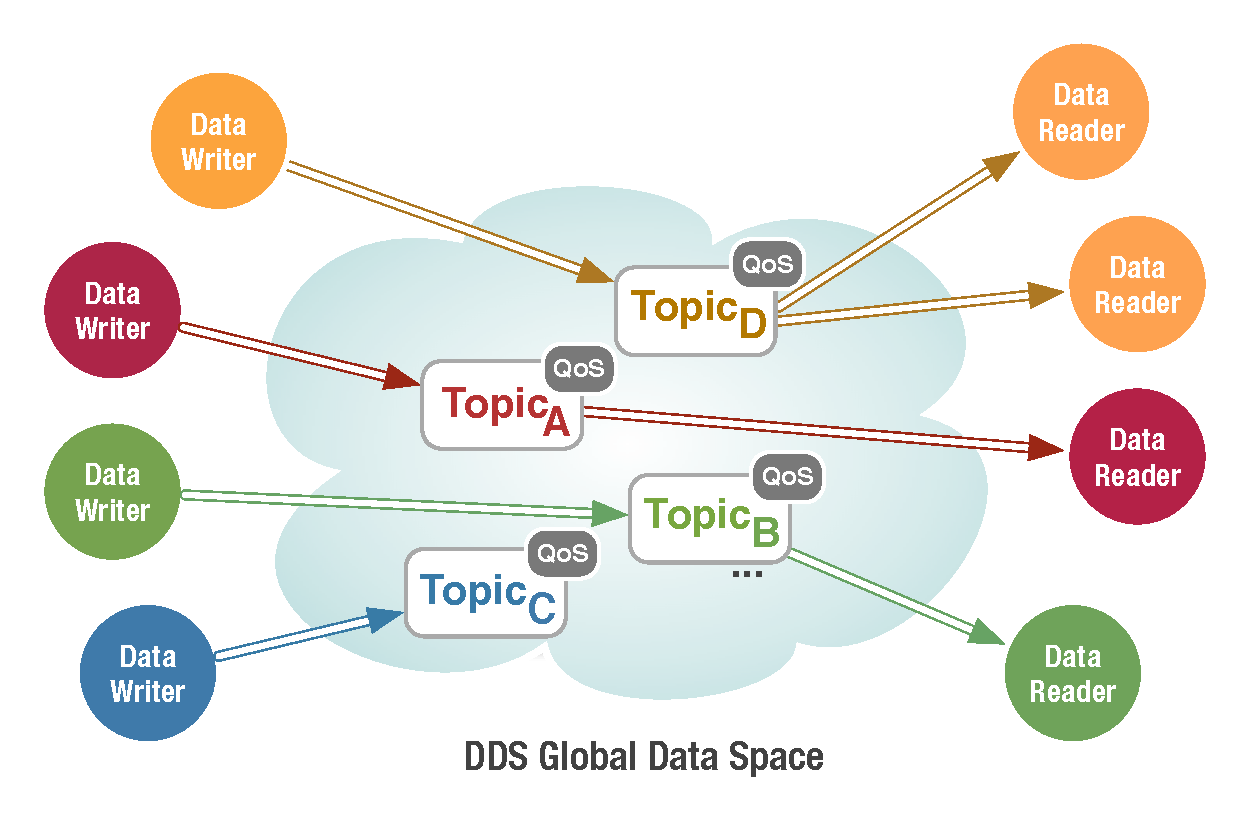
\includegraphics[scale=0.5]{figs/gds.eps}
	\caption{The Global Data Space.}
	\label{Figure:DDS:Standard}
\end{figure}
%%
In essence, the presence of a \ac{GDS} equipped with dynamic discovery 
means that when you deploy a system, you don't have to configure anything. 
Everything will be automatically discovered and data will begin to flow. 
Moreover, since the \ac{GDS} is fully distributed you don't have to fear the 
crash of some server inducing unknown consequences on the system 
availability -- in DDS there is no single point of failure, although 
applications can crash and restart, or connect/disconnect, the system 
as a whole continues to run.

\subsection{Domain Participants}\index{Domain Participant}
To do anything useful a \ac{DDS} application needs to create a \ac{DP}.
The \ac{DP} gives access to the \ac{GDS} -- called domain in \ac{DDS} applications. 
Listing~\ref{Listing:DDS:CreateDP} shows how a \ac{DP} can be created,
notice that domains are identified by integers.

 %%%
\iftoggle{cpp}{
	\lstinputlisting[
		frame=b,
		label={Listing:DDS:CreateDP},
		caption={Topic creation.}]
		{./listing/cxx/create-dp.cpp}
}

%%%
\iftoggle{java}{
	\lstinputlisting[
		frame=b,
		label={Listing:DDS:CreateDP},
		caption={Topic creation.}]
		{./listing/java/create-dp.java}
}
%%%

\iftoggle{scala}{
	\lstinputlisting[
		frame=b,
		label={Listing:DDS:CreateDP},
		caption={Topic creation.}]
		{./listing/scala/create-dp.scala}
}

\subsection{Topics}
I've evoked several times this vision of the data flowing 
from Publishers to Subscribers. In \ac{DDS} this data belongs to a
Topic \index{Topic} and represents the unit of information that can be produced 
or consumed.  A Topic is defined as a triad composed of a type, 
a unique name, and a set of Quality of Service (QoS) policies which, 
as I'll explain in detail later in this tutorial, are used to control 
the non-functional properties associated with the Topic. 
For the time being it is enough to say that if the \ac{QoS}s are not explicitly set, 
then the \ac{DDS} implementation will use some defaults prescribed by the standard.

Topic Types \index{Topic Types} can be represented with the subset of the  \ac{OMG} \ac{IDL}  
standard that defines struct types, with the limitations that Any-types 
are not supported. 
If you are not familiar with the \ac{IDL} standard you should not worry 
as essentially, it is safe for you to think that Topic Types are defined 
with  “C-like” structures whose attributes can be primitive types, 
such as short, long, float, string, etc., arrays, sequences, union 
and enumerations. Nesting of structures is also allowed. On the other hand,
If you are familiar with IDL I am sure you are now wondering how \ac{DDS} 
relates to CORBA. The only things that DDS has in common with CORBA is that 
it uses a subset of IDL; other than this, CORBA and DDS are two completely 
different Standards and two completely different and complementary technologies. 

Now, getting back to our temperature control application, you might want to 
define topics representing the reading of temperature sensors, the conditioners and 
perhaps the rooms in which the temperature sensors and the conditioner are installed. 
Listing~\ref{Listing:IDL:TempSensor} provides an example of how you might define the 
topic type for the temperature sensor.


%%%
\lstinputlisting[frame=b,
                 label={Listing:IDL:TempSensor},
				 caption={The IDL definition for the Temperature Sensor}]
				 {listing/idl/ts.idl}
%%%

As Listing~\ref{Listing:IDL:TempSensor} reveals, \ac{IDL} structures really 
look like C/C++ structures, as a result learning to write Topic Types is usually 
effortless for most programmers.  If you are a "detail-oriented" person you'll 
have noticed that the Listing~\ref{Listing:IDL:TempSensor} also includes a suspicious 
\texttt{ \#pragma keylist} directive. This directive is used to specify keys. The 
\texttt{TempSensorType} is specified to have a single key represented by the 
sensor identifier (id attribute). At runtime, each key value will identify a specific 
stream of data, more precisely, in DDS we say that each key-value identifies a 
Topic instance. For each instance it is possible for you to observe the life-cycle 
and learn about interesting transitions such as when it first appeared in the system, 
or when it was disposed. Keys, along with identifying instances, are also used to 
capture data relationships as you would in traditional entity relationship modeling.  
Keys can be made up by an arbitrary number of attributes, some of which could also 
be defined in nested structures.

After defining the topic type, you can programmatically register \ac{DDS} topic using the \ac{DDS} API by simply instantiating a \texttt{Topic} class with proper type and name.


\iftoggle{cpp}{
	\lstinputlisting[
		frame=b,
		label={Listing:DDS:CreateTopic},
		caption={Topic creation.}]
		{./listing/cxx/create-topic.cpp}
}

\iftoggle{java}{
	\lstinputlisting[
		frame=b,
		label={Listing:DDS:CreateTopic},
		caption={Topic creation.}]
		{./listing/java/create-topic.java}

}

\iftoggle{scala}{
	\lstinputlisting[
		frame=b,
		label={Listing:DDS:CreateTopic},
		caption={Topic creation.}]
		{./listing/scala/create-topic.scala}

}

\subsection{Reading and Writing Data}
\label{Section:ReadWriteData}
Now that you have seen how to specify topics it is time 
to explore how you  can make this Topic flow between 
Publishers and Subscribers. DDS uses the specification 
of user-defined Topic Types to generate efficient encoding and 
decoding routines as well as strongly typed DataReaders and DataWriters. 

Creating a DataReader \index{DataReader} or a DataWriter \index{DataWriter} is straightforward 
as it simply requires you to construct an object by instantiating a 
template class with the Topic Type and passing the desired 
Topic object.  After you've created a DataReader for your 
"TempSensorTopic" you are ready to read the data produced 
by temperature sensors distributed in your system. Likewise after 
you've created a DataWriter for  your “TempSensorTopic” you are 
ready to write (publish) data. Listing~\ref{Listing:DDS:WriteData} and 
\ref{Listing:DDS:ReadData} show the steps required to do so.  

If you look a bit closer at Listing~\ref{Listing:DDS:ReadData}, you'll see that 
our first DDS application is using polling to read data out of DDS every second. 
A sleep  is used to avoid spinning in the loop too fast since the DDS read is 
non-blocking and returns immediately if there is no data available. 
Although polling \index{polling} is a good way to write your first DDS examples it is 
good to know that DDS supports two ways for informing your application 
of data availability, listeners \index{listeners} and waitsets \index{waitsets}. Listeners can be registered 
with readers  for receiving notification of data availability as well as 
several other interesting status changes such as violation in \ac{QoS}.  
Waitsets, modeled after the Unix-style select call, can be 
used to wait the occurrence of interesting events, one of which could 
be the availability of data. I will detail these coordination mechanisms later on
in this tutorial.


\iftoggle{cpp}{
	\lstinputlisting[
		frame=b,
		label={Listing:DDS:WriteData},
		caption={Writing Data in DDS.}]
		{./listing/cxx/write-data.cpp}
}

I think that looking at this code you'll be a bit puzzled since the data 
reader and the data writer are completely decoupled. It is not clear where 
they are writing data to or reading it from, how they are finding about 
each other and so on. This is the DDS magic! As I had explained in the very
beginning of this chapter \ac{DDS} is equipped with dynamic discovery of both 
participants as well as user-defined data types. Thus it is DDS that 
discovers data produces and consumers and takes care of matching them. 
My strongest recommendation is that you try to compile the code examples 
available online (see Appendix A) and run them on your machine 
or even better on a couple of machines. Try running one writer and several 
readers. Then try adding more writers and see what happens. Also experiment
with arbitrary killing (meaning kill -9) readers/writers and restarting them. 
This way you'll see the dynamic discovery in action.


\iftoggle{cpp}{
	\lstinputlisting[
		frame=b,
		label={Listing:DDS:ReadData},
		caption={Reading Data in DDS.}]
		{./listing/cxx/read-data.cpp}
}

\section{Summary}
In this first chapter I've explained the abstraction behind DDS 
and introduced some of its core concepts. I've also shown you 
how to write your first DDS applications that distributes temperature 
sensors values over a distributed system. This was an effort taking  
less than 15 lines of code in total, remarkable, isn't it? In the upcoming 
chapters I'll introduce you to more advanced concepts provided by \ac{DDS} and 
by the end of the series you should be able to use all the \ac{DDS} features 
to create sophisticated scalable, efficient and real-time \ac{Pub/Sub} applications. 

